
% This LaTeX was auto-generated from MATLAB code.
% To make changes, update the MATLAB code and republish this document.

\documentclass{article}
\usepackage{graphicx}
\usepackage{color}

\sloppy
\definecolor{lightgray}{gray}{0.5}
\setlength{\parindent}{0pt}

\begin{document}

    
    \begin{verbatim}
clc, clear all
%%Exercici 1
%a)
A = [1 2 3 4 5];
B = [1; 1; 1; 1; 1];
C = B * A
%b)
A1 = [-1; 0; -1; 2];
B1 = [1 1 1];
C1 = A1 * B1
%%Exercici 2
x = 0:2*pi/30:2*pi;
y = -cos(x);
z = y > 0;
w = y .* z;
figure(1),plot(x,w);
%%Exercici 3
x = -15:1:15;
y = -15:1:15;
[X Y] = meshgrid(x);
f = -((X./7).^2 + (Y./7).^2) + 2;
z = f > 0;
w = f .* z;
figure(3), surf(X,Y,w);
%%Exercici 4
W = [w w; w w];  C = [X-15 X+15; X-15 X+15]; B = [Y+15 Y-15; Y-15 Y+15];
figure(4),surf(C, B, W);


%%Exercici 5
x = -5:0.05:5;
y = -5:0.05:5;
[X Y] = meshgrid(x,y);

f2 = (X.^2+Y-5).^2+(X+Y.^2-9).^2;
figure(5),contour(f2);

[v p] = min(f2); [v1 p1] = min(min(f2)); [p1 p(p1)];
MinimumValue = f2(p(p1),p1)
MinPoint = [(p1-100)*0.05 (p(p1)-100)*0.05]
\end{verbatim}

        \color{lightgray} \begin{verbatim}
C =

     1     2     3     4     5
     1     2     3     4     5
     1     2     3     4     5
     1     2     3     4     5
     1     2     3     4     5


C1 =

    -1    -1    -1
     0     0     0
    -1    -1    -1
     2     2     2


MinimumValue =

    0.0016


MinPoint =

   -2.8500   -3.4000

\end{verbatim} \color{black}
    
\includegraphics [width=4in]{sessio1_01.eps}

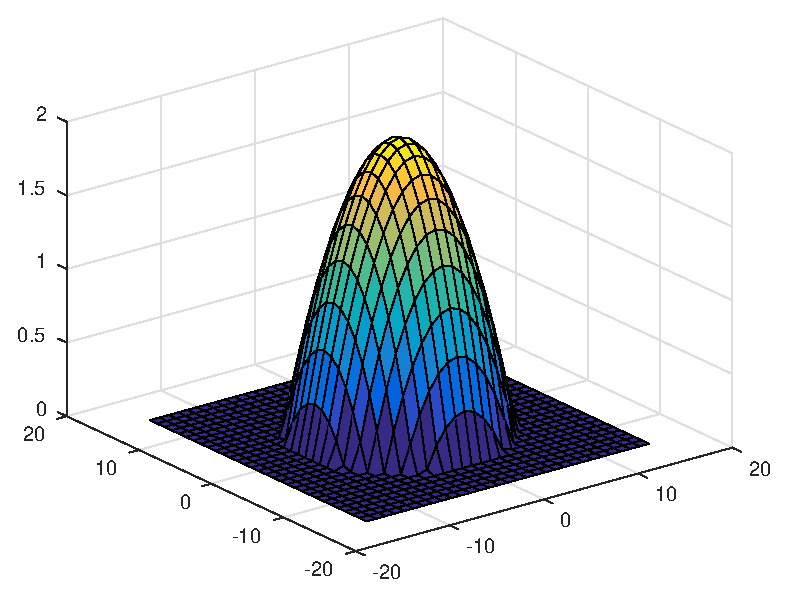
\includegraphics [width=4in]{sessio1_02.eps}

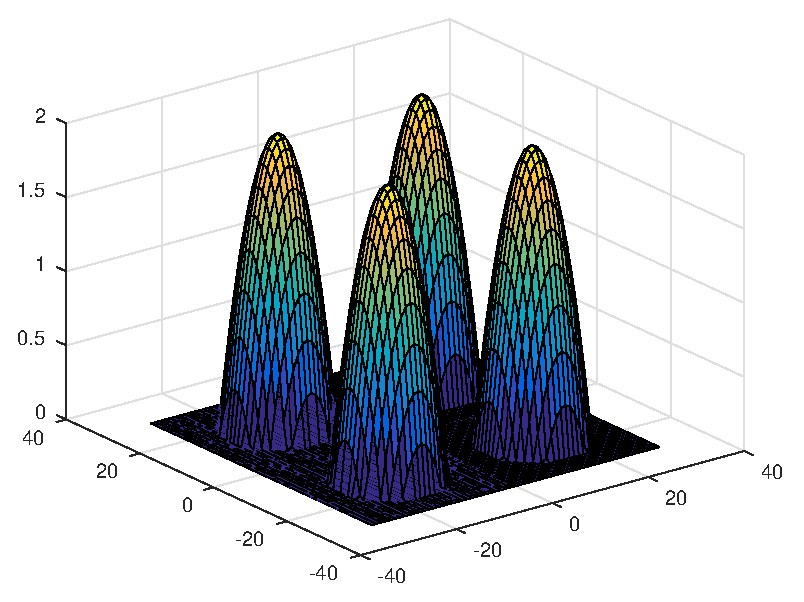
\includegraphics [width=4in]{sessio1_03.eps}

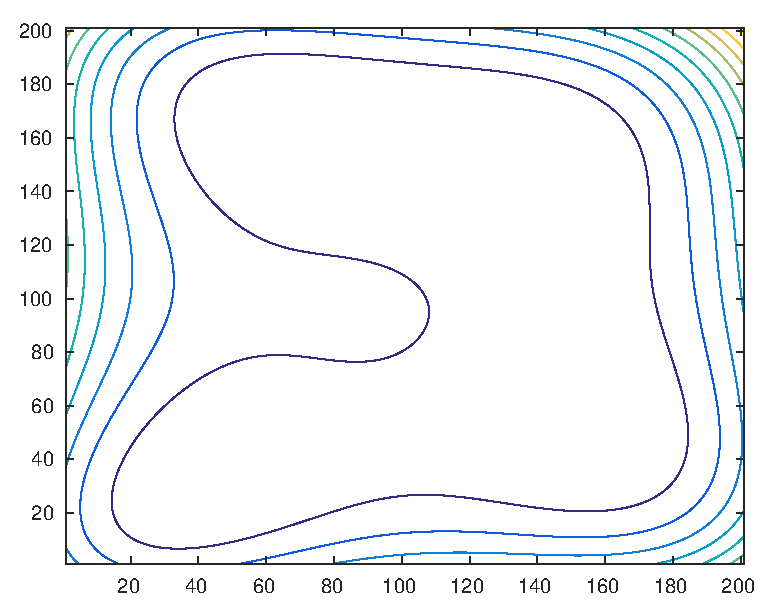
\includegraphics [width=4in]{sessio1_04.eps}



\end{document}
    
